%% =====================================================================
%% Abuse of Autonomous FDIR and Safe Mode in Small Satellites
%% LaTeX source for submission to SpaceSec (co-located with NDSS).
%%
%% TEMPLATE NOTE
%% SpaceSec follows the NDSS template, which is the IEEEtran document
%% class in conference mode (US Letter, two columns, Times 10pt). This
%% file compiles stand-alone with a normal TeX installation. For the
%% camera-ready, download bare_conf_NDSS2027.tex and IEEEtran.cls from
%% the NDSS 2027 templates page, pick the SpaceSec variant (it carries
%% the workshop ISBN and DOI in the footer), and paste the body below
%% into it. Do not change the class options by hand.
%%
%% Build: pdflatex main && pdflatex main   (run twice for references)
%% =====================================================================
\documentclass[conference,letterpaper,10pt]{IEEEtran}

\usepackage[utf8]{inputenc}
\usepackage[T1]{fontenc}
\usepackage{times}
\usepackage{graphicx}
\usepackage{subcaption}
\usepackage{booktabs}
\usepackage{array}
\usepackage{url}
\usepackage{cite}
\usepackage{tikz}
\usetikzlibrary{arrows.meta,positioning,shapes.geometric}
\usepackage[hidelinks]{hyperref}

\graphicspath{{figs/}}

\begin{document}

\title{Abuse of Autonomous FDIR and Safe Mode in\\ Small Satellites: Attack Vectors and Simulated Defenses}

\author{\IEEEauthorblockN{Jose Fabio Navarro Mora}
\IEEEauthorblockA{Independent Researcher\\
Email: fabinho92.fn@gmail.com}}

\maketitle

\begin{abstract}
Small satellites rely on autonomous fault detection, isolation and recovery (FDIR), and on a protective safe mode, so they can survive faults when the ground is out of reach. We show in this paper that the same autonomy can be turned against the mission. Working entirely in simulation, with the NASA Operational Simulator for Small Satellites (NOS3), the core Flight System (cFS) and the COSMOS ground station, we study two attacks on the FDIR and safe mode logic of a representative flight software stack, and we build and measure a defense for each one. One attack needs only a single mode change command, which the baseline software accepts with no authentication, to push the spacecraft into safe mode and stop the science mission. The other forges a low battery reading; the autonomous low power logic then suspends the science by itself, and keeps it suspended for as long as the false value is present. Against the first attack we add an authorization gate on the mode command, and the unauthenticated command is rejected while the legitimate autonomous recovery keeps working. Against the second we add a plausibility gate on the battery telemetry, which holds the last valid value and keeps the science running while the spoof is active. For both cases we report the measured behavior before and after the defense, and we discuss what the defenses do not cover and why authenticated command and telemetry links are the next step.
\end{abstract}

\section{Introduction}
Small satellites operate with little or no contact with the ground for long periods. To survive a fault during these periods, the flight software runs an autonomous fault management function, usually called FDIR (fault detection, isolation and recovery), together with a safe mode. FDIR watches the health telemetry, detects a bad condition, and runs a stored recovery sequence. Safe mode is a reduced state where the satellite stops the mission activity, points to the Sun, and waits for the operator. This autonomy is what keeps the spacecraft alive, so it is given a lot of authority over the vehicle.

The problem is that this authority sits on two trust boundaries that are often weak. The first boundary is the command link: if a mode change command is accepted without authentication, anyone who can inject a command can move the satellite into safe mode. The second boundary is the health telemetry: if the FDIR acts on a single sensor reading without validating it, a forged or stuck reading can drive the recovery logic. In both cases the attacker does not need to break the satellite, the attacker only needs to make the satellite protect itself at the wrong time.

We make this concrete in this paper. We demonstrate two attacks on the FDIR and safe mode logic of a representative flight software stack, and we build and measure a defense for each. One attack abuses an unauthenticated mode change command. The other drives the autonomous low power response by forging a low battery reading. Both map to the SPARTA framework (technique EX-0011, exploit reduced protection during safe mode), and we design the first defense after the SPARTA countermeasure CM0044, cyber safe mode. Our contribution is not a new cryptographic protocol. It is a clear and reproducible demonstration of the two attacks, together with two low cost defenses and their measured before and after behavior.

The scope of this work is defensive and academic. Everything runs inside the NOS3 simulator on open source NASA software. No real satellite or real ground system is involved. If we find a real vulnerability in the open source code, we follow responsible disclosure, as described in Section~\ref{sec:disclosure}.

\section{Background}

\subsection{NOS3, cFS and COSMOS}
NOS3 (NASA Operational Simulator for Small Satellites) is an open source simulation environment for small satellite flight software~\cite{nos3}. It runs the real flight software on top of the core Flight System (cFS)~\cite{cfs}, together with simulated hardware and a simulated space dynamics model (42). The ground side uses COSMOS, which provides a command sender and a telemetry viewer. Because NOS3 runs the real cFS applications and the real onboard tables, an attack or a defense that works in NOS3 is close to what would happen on a comparable flight build. This makes NOS3 a good and safe place to study the security of the autonomy logic.

\subsection{The FDIR chain}
In this flight software, the autonomous fault management is built from four cFS pieces that form a chain. The Electrical Power System application (GENERIC\_EPS) and the other device applications publish health telemetry, for example the battery voltage. The Limit Checker application (LC) holds a table of watchpoints, where each watchpoint compares one telemetry field against a threshold. When a watchpoint becomes true, it feeds an actionpoint in a second table. An actionpoint combines one or more watchpoints with a simple logic equation, and when its condition is met it triggers a stored command sequence, called a Relative Time Sequence (RTS), inside the Stored Command application (SC). The RTS then sends the commands that perform the recovery, for example a command to the manager application (MGR) that changes the spacecraft mode. The manager application keeps the spacecraft mode and the science status, and it reports them in its housekeeping telemetry.

So the full chain is telemetry, then watchpoint, then actionpoint, then RTS, then a command back to the manager or to other applications. The important point for security is that each step trusts the previous one. The watchpoint trusts the telemetry. The RTS trusts the actionpoint. The manager trusts the command it receives.

\begin{figure}[t]
\centering
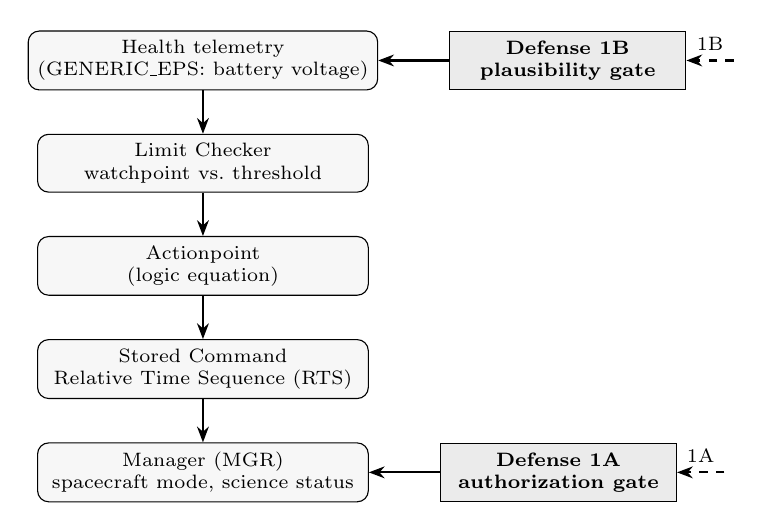
\begin{tikzpicture}[
  node distance=5.5mm,
  box/.style={draw, rounded corners, align=center, font=\scriptsize,
              minimum width=42mm, minimum height=7mm, fill=black!3},
  gate/.style={draw, align=center, font=\scriptsize\bfseries,
               minimum width=30mm, minimum height=6mm, fill=black!8},
  flow/.style={-{Stealth[length=2mm]}, thick},
  atk/.style={-{Stealth[length=2mm]}, thick, dashed}
]
\node[box] (tlm)  {Health telemetry\\(GENERIC\_EPS: battery voltage)};
\node[box, below=of tlm] (lc)   {Limit Checker\\watchpoint vs.\ threshold};
\node[box, below=of lc]  (ap)   {Actionpoint\\(logic equation)};
\node[box, below=of ap]  (rts)  {Stored Command\\Relative Time Sequence (RTS)};
\node[box, below=of rts] (mgr)  {Manager (MGR)\\spacecraft mode, science status};

\draw[flow] (tlm) -- (lc);
\draw[flow] (lc)  -- (ap);
\draw[flow] (ap)  -- (rts);
\draw[flow] (rts) -- (mgr);

% Defense 1B gate on telemetry (top)
\node[gate, right=9mm of tlm] (g1b) {Defense 1B\\plausibility gate};
\draw[atk] ([xshift=6mm]g1b.east) -- node[above, font=\scriptsize] {1B} (g1b.east);
\draw[flow] (g1b.west) -- (tlm.east);

% Defense 1A gate on command (bottom)
\node[gate, right=9mm of mgr] (g1a) {Defense 1A\\authorization gate};
\draw[atk] ([xshift=6mm]g1a.east) -- node[above, font=\scriptsize] {1A} (g1a.east);
\draw[flow] (g1a.west) -- (mgr.east);
\end{tikzpicture}
\caption{The FDIR chain, with the two attack points and the two defenses. The chain runs from the health telemetry down to the manager. Vector 1B injects a false reading at the top of the chain, and vector 1A injects an unauthenticated command at the bottom. Defense 1B gates the telemetry and defense 1A gates the command.}
\label{fig:fdir}
\end{figure}

\subsection{Safe mode and the low power response}
The manager application defines four modes: safe, safe reboot, science and science reboot. Safe mode is the protective state. The spacecraft also has an autonomous low power response: when the battery voltage drops below a threshold, the FDIR chain suspends the science activity and sets the science status to a low power value. This is a graceful degradation, not a full safe mode, but for the mission it has the same effect, the science stops.

\subsection{SPARTA}
SPARTA (Space Attack Research and Tactic Analysis) is a public framework~\cite{sparta} that describes attacker techniques and countermeasures for space systems. Our first attack maps to technique EX-0011, exploit reduced protection during safe mode, because it forces the vehicle into a reduced state on demand. Our first defense follows the countermeasure CM0044, cyber safe mode, which asks for an authenticated and authorized path before the vehicle changes into a protective mode.

\section{Threat model}
We assume an attacker who can place data on one of the two input paths of the spacecraft, but who cannot change the flight software itself. We consider two capabilities, and each attack uses only one of them.

For the first attack, the attacker can inject a command into the command link. This models a compromised or spoofed ground segment, a replayed command, or any situation where the uplink is not authenticated. The attacker does not need to know any secret, because in the baseline system the mode command is accepted without authentication.

For the second attack, the attacker can inject or alter a telemetry value that the FDIR reads, in our case the battery voltage. This models a compromised sensor bus, a forged telemetry packet, or a manipulated sensor. In the simulator we produce this condition through the simulation input path, which gives the same effect as a false reading arriving at the flight software.

The following items are out of scope. We do not consider physical attacks on the hardware, attacks that modify the flight software binary or the onboard tables, denial of service against the radio link itself, or attacks on the ground network outside the command and telemetry path. We also assume that the operator cannot keep a continuous contact with the spacecraft, which is the normal situation for a small satellite and which is what makes a persistent autonomous effect so damaging.

\section{Attack vectors}

\subsection{Vector 1A: unauthenticated mode change}
The manager application changes the spacecraft mode through the command \texttt{MGR\_SET\_MODE\_CC}. In the baseline flight software, the handler of this command only checks the length of the message and the range of the mode value (one to four). It does not check the origin of the command and it does not ask for any authorization. Any command with the correct format is applied.

The attack is therefore a single command. The attacker sends \texttt{MGR\_SET\_MODE\_CC} with the value for safe reboot. The manager applies it, the command error count does not increase, and the spacecraft leaves the science mode. The operator can command the science mode again, so this denial of service is reversible, but each unauthenticated command is enough to interrupt the mission.

\subsection{Vector 1B: forged low battery telemetry}
The low power branch of the FDIR works as follows. Watchpoint 27 compares the battery voltage field of the EPS housekeeping against a low threshold. When the battery voltage is below the threshold, watchpoint 27 becomes true, actionpoint 27 triggers RTS 27, and RTS 27 suspends the science activity and sets the science status to the low power value. A second watchpoint, number 28, is the recovery condition, and it becomes true only when the battery voltage goes above a higher threshold, which represents a well charged battery.

The attack forges a low battery reading. When the reported battery voltage drops below the low threshold, the FDIR suspends science on its own, with no mode command at all. The key property is the recovery condition: science resumes only when the battery reads as well charged. So if the attacker keeps the battery reading low, the recovery never triggers, and the science never resumes. This is a persistent denial of service, and it is stronger than vector 1A, because the operator cannot recover the mission by commanding the science mode while the false reading is present. The satellite fights against its own operator, which is the behavior described by SPARTA EX-0011.

An important observation from our analysis is that, in the reference FDIR configuration of this flight software, there is no autonomous path from low battery to full safe mode. The autonomous response to low power is the graceful degradation above. Full safe mode is entered only by a startup sequence or by the mode command of vector 1A. We keep this distinction in the paper because it changes the shape of the two denial of service effects.

\section{Experimental setup}
We run NOS3 with its standard single spacecraft configuration. The flight software is cFS with the manager, Limit Checker, Stored Command and EPS applications described above. The ground side is COSMOS, where we use the Command Sender to send commands and the Packet Viewer to read telemetry.

We observe two housekeeping packets. From the manager packet (\texttt{MGR\_HK\_TLM}) we read the spacecraft mode, the science status, the command count and the command error count. From the EPS packet (\texttt{GENERIC\_EPS\_HK\_TLM}) we read the battery voltage and the solar array voltage. We also read the cFS event console, which prints the events of each application, because the events show the internal decisions of the FDIR chain and of our defenses.

For vector 1A we send the mode command from the COSMOS Command Sender. For vector 1B we need to change a sensor value, so we use the NOS Terminal, which is the simulation command interface that NOS3 opens together with the system. Through the NOS Terminal we set the EPS simulation node and write a lower state of charge, which makes the simulated battery report a lower voltage. This is our injection point for a false low battery reading.

For each experiment we record a baseline, then we apply the attack, and then we read the same telemetry again. For the defenses we repeat the same attack after the defense is built, so we can compare the before and the after under the same conditions. The flight software is rebuilt with the NOS3 build flow (\texttt{make config}, \texttt{make fsw}, \texttt{make launch}), which regenerates the applications and the onboard tables.

\section{Attack results}

\subsection{Vector 1A}
Starting from the science mode, we sent one \texttt{MGR\_SET\_MODE\_CC} command with the safe reboot value. The manager accepted it and the spacecraft mode changed to safe reboot. The command count increased by one and the command error count stayed at zero, which confirms that the command was accepted as valid, with no origin check and no authorization. Commanding the science mode again returned the spacecraft to science, so the effect is reversible but repeatable.

\subsection{Vector 1B}
Starting from the science mode with the battery near 25.2 volts, we wrote a lower state of charge through the NOS Terminal. The reported battery voltage dropped to about 24.0 volts, below the low threshold. Watchpoint 27 became true, actionpoint 27 triggered RTS 27, and the science status changed to the low power value. The science activity was suspended with no mode command involved. Because the recovery watchpoint only becomes true when the battery reads as well charged, the science stayed suspended while the low reading was present. This is the persistent denial of service.

\subsection{Summary}
Table~\ref{tab:attacks} summarizes the two effects.

\begin{table}[t]
\caption{Summary of the two attack vectors}
\label{tab:attacks}
\centering
\footnotesize
\begin{tabular}{@{}p{14mm}p{18mm}p{22mm}p{16mm}@{}}
\toprule
Vector & Input used & Observed effect & Recovery \\
\midrule
1A unauthenticated mode command & one \texttt{MGR\_SET\_MODE\_CC} to safe reboot & spacecraft leaves science, command error count stays at zero & reversible, operator can command science again \\
\addlinespace
1B forged low battery & lower state of charge, battery reads low & science status becomes low power, science suspended with no command & persistent, blocked while the false reading is held \\
\bottomrule
\end{tabular}
\end{table}

\section{Defenses}

\subsection{Defense 1A: authorization gate on the mode command}
The first defense adds an authorization gate to the mode command, following the idea of SPARTA CM0044. We extend the mode command with an authorization token and we change the manager handler so that it applies the mode change only when the token is valid. A command without a valid token is rejected, the command error count increases, and the mode does not change. The handler also keeps the previous length and range checks.

The important design point is that the mode command is also used by the spacecraft itself. The autonomous recovery sequence RTS 025 sends a mode command to return from science reboot to science. If we only protect the handler, we would break this legitimate internal use. For this reason we also update RTS 025 so that it carries the valid token. This keeps the autonomous recovery working while the external unauthenticated command is blocked.

We implement the token as a single static byte. We are explicit that this is a reference implementation of the gate, not real cryptography. It shows the place and the logic of the check. An operational version would use an authenticated command link, for example CCSDS SDLS~\cite{sdls} with a message authentication code for each command, instead of a static token. We discuss this in Section~\ref{sec:limits}.

\subsection{Defense 1B: plausibility gate on the battery telemetry}
The second defense adds a plausibility gate to the battery telemetry inside the EPS application, before the housekeeping is published. The gate keeps the last valid battery voltage. If a new reading drops by more than a physical slew limit in one sample, and this drop is not corroborated by a drop of the solar array voltage, the gate marks the reading as suspect. For a suspect reading the gate holds the last valid value in the published telemetry, so the Limit Checker watchpoint reads the held value and does not trigger. The gate also increases a suspect counter and sends a cFS event, so the attempt is visible to the operator instead of being silent.

The slew limit encodes a simple physical fact, a real battery cannot lose a large part of its voltage between two telemetry samples that are a few seconds apart. The solar cross check is used only to relax the gate, that is, a sharp drop that is corroborated by the solar array is treated as a possible real power event and is not held. This direction avoids false holds during a genuine power problem.

This defense does not change the offset of the battery voltage field and does not change the ground telemetry definition, so the existing watchpoint benefits from the sanitized value with no table change. As with defense 1A, this is a resilience and detection control, not an authentication control, and we state its limits in Section~\ref{sec:limits}.

\section{Defense evaluation}

\subsection{Defense 1A}
We measured three cases after building the gate. In case A we sent the mode command with an invalid token (zero). The command was rejected, the command error count increased, the mode did not change, and the console printed the rejection event. In case B we sent the mode command with the valid token. The command was accepted and the mode changed, which shows that an authorized change still works. In case C we checked the autonomous recovery. The FDIR chain triggered RTS 025, and the internal mode command of RTS 025, now carrying the token, was accepted with no length error, so the autonomous recovery still returns the spacecraft to science.

\begin{table}[t]
\caption{Defense 1A: measured cases}
\label{tab:def1a}
\centering
\footnotesize
\begin{tabular}{@{}p{5mm}p{22mm}p{14mm}p{24mm}@{}}
\toprule
Case & Command & Expected & Observed \\
\midrule
A & mode command, invalid token & rejected & rejected, command error count increased, mode unchanged \\
\addlinespace
B & mode command, valid token & accepted & accepted, mode changed to science \\
\addlinespace
C & autonomous RTS 025 with token & accepted & RTS 025 triggered, internal mode command accepted, no length error \\
\bottomrule
\end{tabular}
\end{table}

During this evaluation we also found a practical lesson. Adding the token changes the length of the authenticated command. If the flight software application is rebuilt but the stored command tables are not regenerated, the table still sends the old, shorter command, and the manager rejects the internal command of RTS 025 because of the wrong length. In that intermediate state the autonomous recovery is broken and the mode stays in science reboot. The conclusion is that this kind of defense must update the application, the stored command tables, and the ground definitions together. If an operator patches only the application, a security hardening turns into an availability regression of the FDIR.

\begin{figure}[t]
\centering
\begin{subfigure}{\columnwidth}
  \centering
  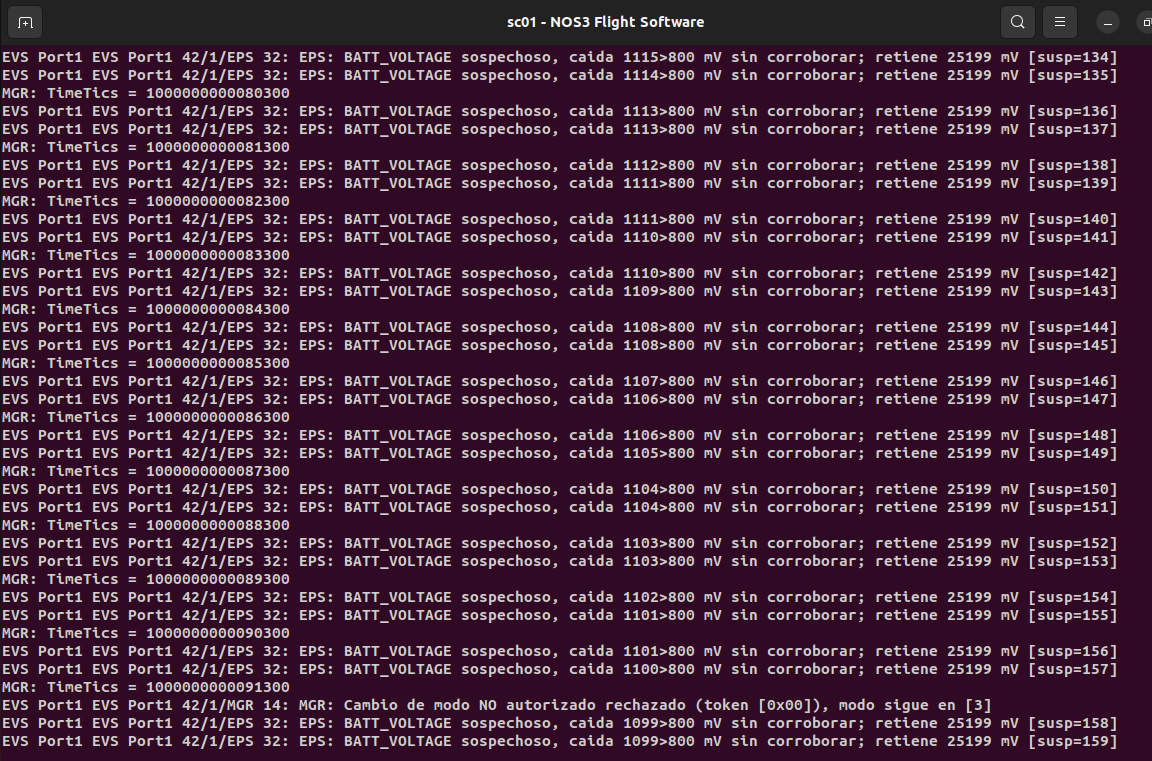
\includegraphics[width=\columnwidth]{fig2a_1A_console.png}
  \caption{The manager rejects the mode command that carries an invalid token and prints the rejection event, so the mode stays in science.}
\end{subfigure}
\\[2mm]
\begin{subfigure}{\columnwidth}
  \centering
  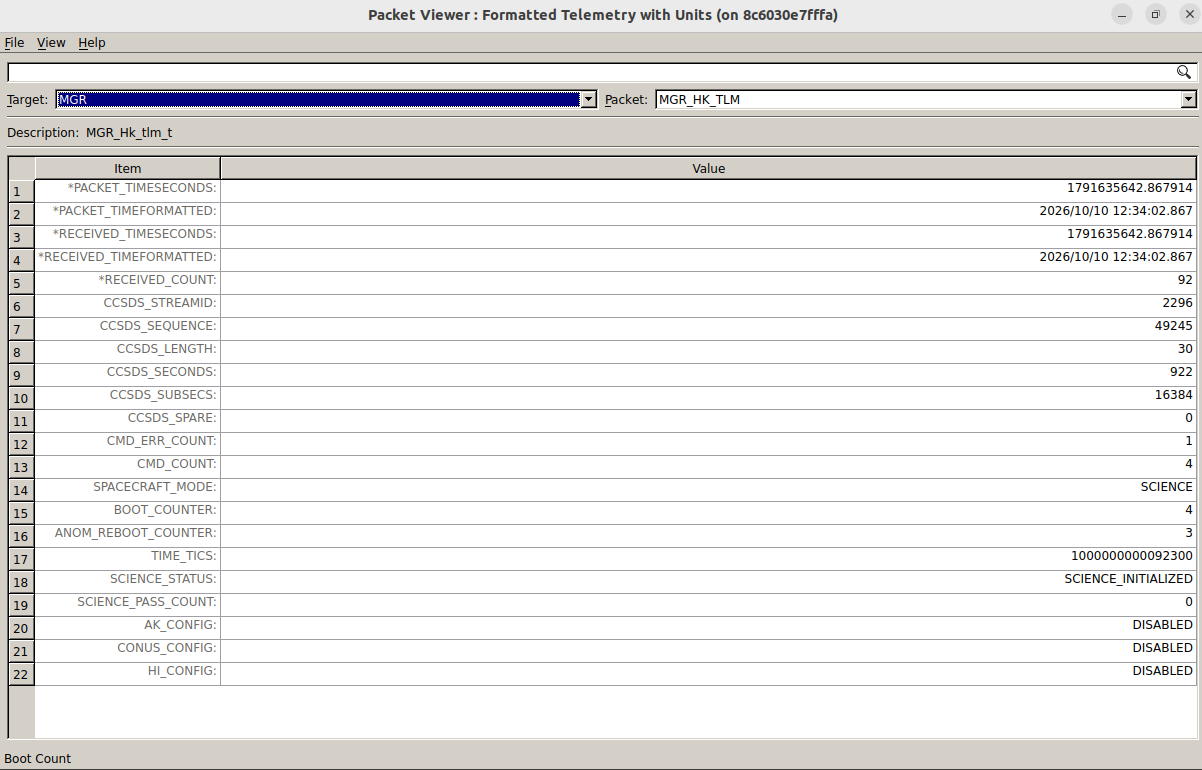
\includegraphics[width=\columnwidth]{fig2b_1A_mgr_hk.png}
  \caption{The spacecraft mode stays SCIENCE and the command error count records the rejected command, so the unauthenticated command has no effect.}
\end{subfigure}
\caption{Defense 1A under the unauthorized mode command (case A).}
\label{fig:def1a}
\end{figure}

\subsection{Defense 1B}
We enabled the science mode, which also arms the low power monitor (actionpoint 27), and then we ran the same forged low battery attack as in vector 1B. With the defense in place, the console printed a series of events of the form battery voltage suspect, drop above the slew limit, not corroborated, holding the last valid value, with a growing suspect counter. The published battery voltage stayed at about 25.2 volts and never reached the low value. The science status stayed at the initialized value, so the science was not suspended. The low power monitor was armed, and the autonomous FDIR kept working normally, only the poisoned reading was blocked.

\begin{table}[t]
\caption{Defense 1B: before and after}
\label{tab:def1b}
\centering
\footnotesize
\begin{tabular}{@{}p{20mm}p{24mm}p{22mm}@{}}
\toprule
Scenario & Published battery voltage & Science status \\
\midrule
Without defense & drops to about 24.0 V & low power, science suspended \\
\addlinespace
With defense 1B & held at about 25.2 V & initialized, science active \\
\bottomrule
\end{tabular}
\end{table}

The attack in our test was a single write, and the simulated battery recharges from the solar array, so the drop slowly becomes smaller while the state of charge returns. The gate held the value during the whole dip. A sustained attack, where the attacker keeps writing the low value, would be rejected in the same way at each sample, because each reading is compared against the held valid value.

\begin{figure}[t]
\centering
\begin{subfigure}{\columnwidth}
  \centering
  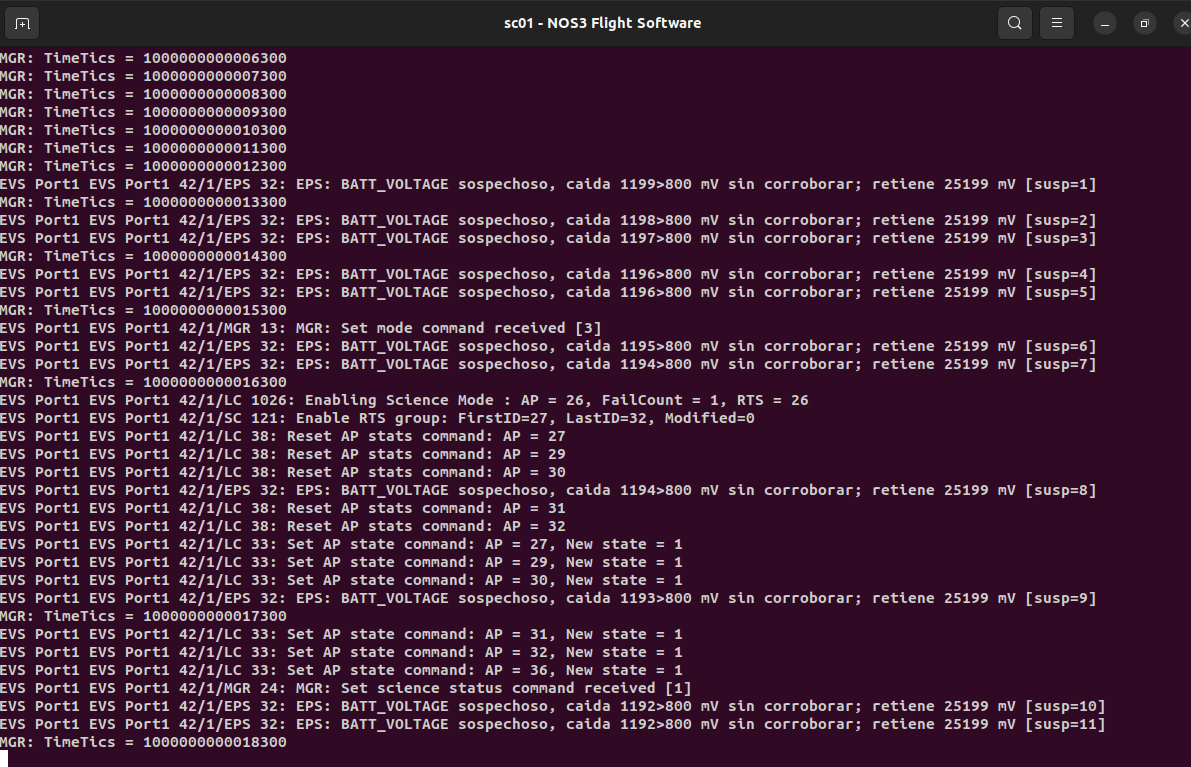
\includegraphics[width=\columnwidth]{fig3a_1B_console.png}
  \caption{The EPS plausibility gate marks each suspect reading, holds the last valid value, and increases a suspect counter.}
\end{subfigure}
\\[2mm]
\begin{subfigure}{0.78\columnwidth}
  \centering
  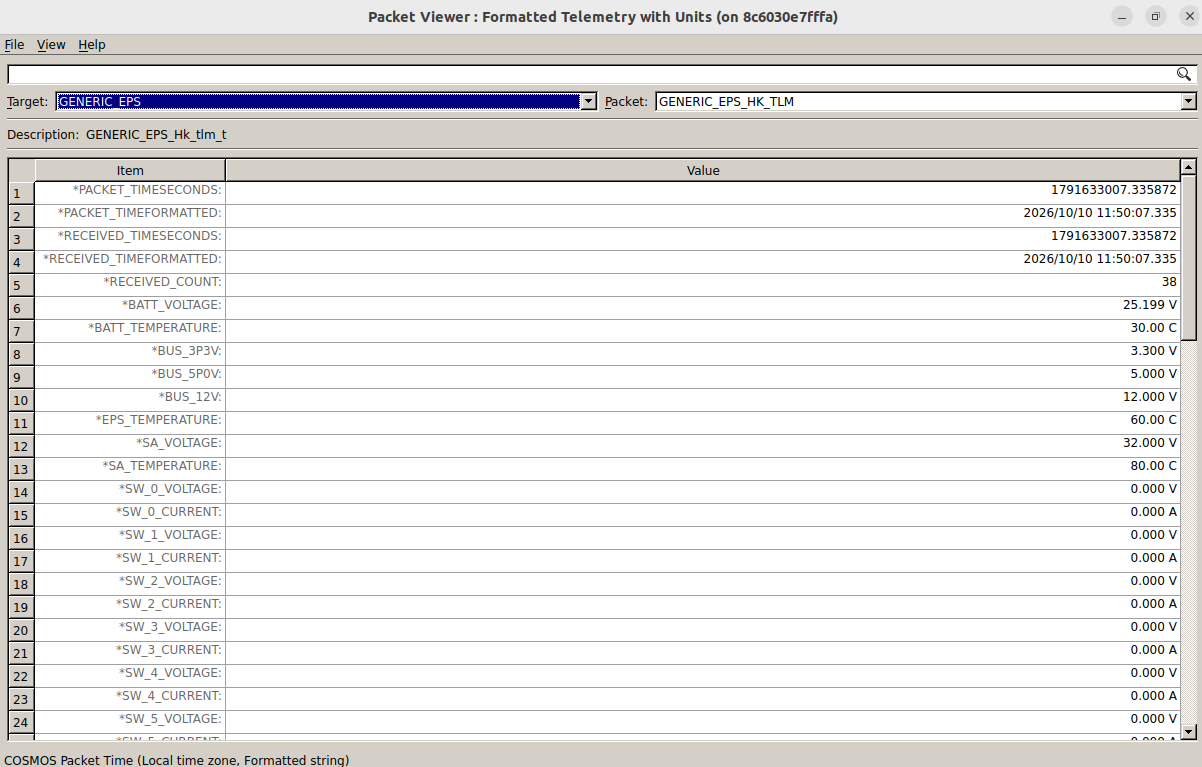
\includegraphics[width=\columnwidth]{fig3b_1B_eps.png}
  \caption{The published battery voltage stays at 25.199 V and never reaches the low threshold.}
\end{subfigure}
\\[2mm]
\begin{subfigure}{0.78\columnwidth}
  \centering
  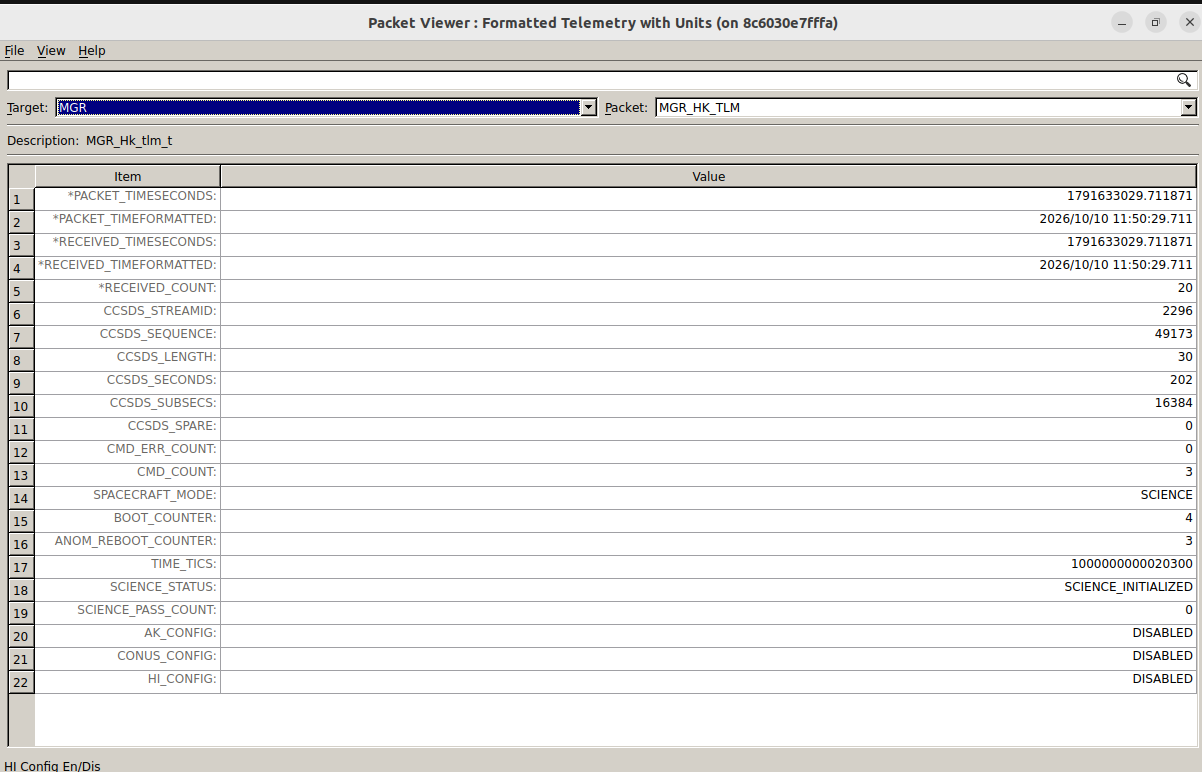
\includegraphics[width=\columnwidth]{fig3c_1B_mgr.png}
  \caption{The spacecraft stays in science and the science status stays initialized, so the mission is not suspended.}
\end{subfigure}
\caption{Defense 1B under the forged low battery attack.}
\label{fig:def1b}
\end{figure}

\section{Limitations and future work}
\label{sec:limits}
Our defenses are intentionally simple, and they have clear limits. The authorization token of defense 1A is a single static byte, so it is not real cryptography. It shows where the authorization check belongs and that the check does not break the autonomy, but a static token can be read or replayed. The plausibility gate of defense 1B is a detection and resilience control, not an authentication control. It stops an instantaneous spoof and it raises an alert, but an attacker who lowers the value slowly, inside the slew limit, could still move the reading down over time. Neither defense proves the origin of the data.

Our evaluation also uses a single simulator and a single reference configuration. The reference FDIR tables of this flight software may differ from the tables of a real mission, in particular the low power branch uses graceful degradation and not a full safe mode. For vector 1B, we produce the false reading through the simulation input, which keeps the battery voltage and the state of charge consistent. A direct forgery of only the voltage field on the bus would be even easier to detect with the solar cross check, so our test is a conservative case for the defense.

Future work goes in three directions. First, replace the static token with an authenticated command link, for example CCSDS SDLS with a message authentication code per command, and measure the cost on the onboard processor. Second, extend the plausibility idea to authenticated or signed telemetry, and add an operator acknowledgment step before the FDIR performs a safing action that stops the mission. Third, apply the same method to more FDIR branches and more sensors, and study how a defense in depth that combines authentication, plausibility and operator confirmation behaves against a wider set of attacks.

\section{Responsible disclosure}
\label{sec:disclosure}
This work uses open source NASA software (NOS3 and cFS) and studies its reference configuration. The attacks we show rely on design properties of the reference setup, for example a mode command that is accepted without authentication and an FDIR branch that acts on a single telemetry field. These are not secret and they are visible in the public source and tables.

If during this research we identify a specific vulnerability in the open source code, rather than a configuration or design property that is already public, we report it to the maintainers through their stated channels before any public description, and we give them reasonable time to respond. We do not publish any exploit against a real system, and all of our testing stays inside the simulator. Our goal is to help mission designers and the open source community, so we share our defenses and our measurements together with the attacks.

\section{Related work}
Our work sits in three lines of research. The first line studies the security of real satellite and spacecraft software, including analysis of flight software images and of the weak authentication of command and telemetry links~\cite{spaceodyssey}. This line shows that many onboard systems trust commands and data with little or no verification, which is the same assumption we use in our threat model. The second line studies the space link itself, including eavesdropping and spoofing of satellite signals~\cite{vsat}, and the general lack of integrity protection in older link protocols. The third line is the set of community frameworks and standards, in particular the SPARTA framework for space attacker techniques and countermeasures~\cite{sparta}, and the CCSDS Space Data Link Security (SDLS) standard for authenticated command links~\cite{sdls}.

A fourth and very recent line uses the same NOS3 and cFS environment that we use, which lets us compare directly. Vanlyssel et al.\ demonstrate onboard sensor spoofing through a supply chain implant~\cite{silentsub} and multi-vector supply chain attacks that reach denial of service~\cite{spychain}, both inside NOS3, and a recent taxonomy of satellite cybersecurity~\cite{satsok} maps the broader threat space. These works show that false telemetry and malicious onboard components are practical in this simulator, and they point to robust fault management and cyber safe mode as countermeasures, but they do not target the FDIR chain itself and they do not implement or measure such a defense. This is the specific gap we fill.

Our contribution is complementary. Instead of analyzing a single real firmware or a single link, we focus on the autonomy itself, that is the FDIR and safe mode logic, and we show two concrete ways to abuse it and two defenses, all reproducible in an open source simulator. To our knowledge, the abuse of the FDIR chain and of the autonomous low power response, together with a measured defense for each, is not covered in detail in the current literature.

\section{Conclusion}
The autonomy that keeps a small satellite alive can also work against the mission. We showed two attacks on the FDIR and safe mode logic of a representative open source flight software stack. One uses a single unauthenticated mode command to leave the science mode. The other forges a low battery reading, and the autonomous low power response then suspends the science, and keeps it suspended, with no command at all. For each attack we built and measured a defense, an authorization gate on the mode command and a plausibility gate on the battery telemetry, and in both cases the defense stopped the attack while the legitimate autonomy kept working.

The main lesson for mission designers is simple. The FDIR and the safe mode must treat both the commands and the health telemetry as inputs that can be wrong or hostile. A command that changes the vehicle state should be authenticated and authorized, and a sensor value that can stop the mission should be validated before the autonomy acts on it. Our defenses are only a first step toward this, but they show that the checks can be added at a low cost and without breaking the autonomy, which is the property that matters for a real mission.

\begin{thebibliography}{9}
\bibitem{spaceodyssey}
J. Willbold, M. Schloegel, M. V\"ogele, M. Gerhardt, T. Holz, and A. Abbasi,
``Space Odyssey: An Experimental Software Security Analysis of Satellites,''
in \emph{2023 IEEE Symposium on Security and Privacy (S\&P)}, 2023, pp. 1--19.
doi: 10.1109/SP46215.2023.10351029.

\bibitem{vsat}
J. Pavur, D. Moser, M. Strohmeier, V. Lenders, and I. Martinovic,
``A Tale of Sea and Sky: On the Security of Maritime VSAT Communications,''
in \emph{2020 IEEE Symposium on Security and Privacy (S\&P)}, 2020, pp. 1384--1400.
doi: 10.1109/SP40000.2020.00056.

\bibitem{sparta}
The Aerospace Corporation,
``SPARTA: Space Attack Research and Tactic Analysis,''
\url{https://sparta.aerospace.org/}. Accessed 2026.

\bibitem{sdls}
Consultative Committee for Space Data Systems,
``Space Data Link Security Protocol,''
CCSDS 355.0-B-2, Blue Book, 2022.

\bibitem{nos3}
M. Suder,
``NOS3: NASA Operational Simulator for Small Satellites,''
in \emph{Flight Software Workshop (FSW)}, 2018. Software catalog GSC-17737-1.
\url{https://nos3.readthedocs.io/}.

\bibitem{cfs}
D. McComas,
``NASA/GSFC's Flight Software Core Flight System,''
in \emph{Flight Software Workshop (FSW)}, 2012.

\bibitem{silentsub}
J. Vanlyssel, G.-C. Roman, and A. Anwar,
``Silent Subversion: Sensor Spoofing Attacks via Supply Chain Implants in Satellite Systems,''
arXiv:2603.10388, 2026.

\bibitem{spychain}
J. Vanlyssel, E. Sobrados, R. Anwar, G.-C. Roman, and A. Anwar,
``SpyChain: Multi-Vector Supply Chain Attacks on Small Satellite Systems,''
arXiv:2510.06535, 2025.

\bibitem{satsok}
R. Peled, E. Aizikovich, E. Habler, Y. Elovici, and A. Shabtai,
``Rethinking Satellite Cybersecurity: A System-Level Taxonomy and Longitudinal Analysis,''
arXiv:2312.01330, 2023.
\end{thebibliography}

\end{document}
